\documentclass[journal]{IEEEtran}

\usepackage{cite}
\usepackage{amsmath,amssymb,amsfonts,amsthm}
\usepackage{algorithmic}
\usepackage{graphicx}
\usepackage{textcomp}
\usepackage{xcolor}
\usepackage{booktabs}
\usepackage{microtype}
\usepackage{url}

% Float and space compaction for exact 6-page calibration
\setlength{\textfloatsep}{7pt plus 1pt minus 1pt}
\setlength{\floatsep}{6pt plus 1pt minus 1pt}
\setlength{\intextsep}{6pt plus 1pt minus 1pt}
\setlength{\dbltextfloatsep}{7pt plus 1pt minus 1pt}
\setlength{\dblfloatsep}{6pt plus 1pt minus 1pt}
\setlength{\abovecaptionskip}{3pt}
\setlength{\belowcaptionskip}{3pt}

% Theorem environments
\newtheorem{theorem}{Theorem}
\newtheorem{lemma}{Lemma}
\newtheorem{corollary}{Corollary}
\newtheorem{definition}{Definition}
\newtheorem{remark}{Remark}

\begin{document}

\title{Exact One-Electron Diagnostics, Symmetry-Breaking Bifurcations, and Order-Theoretic Structure of Machine-Learned Exchange--Correlation Functionals}

\author{Dalton~Omondi%
\thanks{D. Omondi is an independent researcher in Computational Chemistry and Mathematical Physics, Nairobi, Kenya (e-mail: daltonomondi588@gmail.com).}%
\thanks{All source code, convergence logs, master datasets ($N=96$ calculations), and figure generation pipelines are openly archived at \protect\url{https://github.com/GabuGravin41/dftex-func-}.}
}

\markboth{IEEE Transactions on Molecular \& Quantum Engineering,~Vol.~XX, No.~X,~October~2026}%
{Omondi: One-Electron Diagnostics, Bifurcations, and Order Theory in ML-XC}

\maketitle

\begin{abstract}
Machine-learned exchange--correlation (ML-XC) functionals have rapidly emerged as flexible, highly accurate approximations for molecular and solid-state ground-state energetics. However, their reliance on empirical multi-electron datasets frequently obscures severe physical pathologies in one-electron and asymptotic regimes. In this work, we construct a rigorous, zero-parameter one-electron computational diagnostic framework to probe self-interaction error (SIE), fractional-charge delocalization, and orbital stability in representative standard and machine-learned functionals. First, we demonstrate that traditional benchmarks referencing infinite-basis hydrogenic eigenvalues ($-Z^2/2$) artificially inflate one-electron SIE by 30--66\% due to contracted Gaussian basis-set incompleteness. By evaluating against an exact same-basis unrestricted Hartree--Fock (UHF) reference across four standard Gaussian basis sets (\texttt{def2-SVP}, \texttt{def2-TZVP}, \texttt{def2-QZVP}, and \texttt{aug-cc-pVTZ}), we completely eliminate basis artifacts and isolate pure functional errors across five functional classes (PBE, r2SCAN, SCAN, B3LYP, and CIDER). Second, through a 16-point internuclear separation scan of the stretched $\text{H}_2^+$ molecular ion, we definitively verify the existence of a symmetry-breaking bifurcation: approximate semilocal and hybrid functionals undergo an orbital stability transition at $R_c \approx 5.5\text{--}6.0\ \text{\AA}$, where the physical symmetric ground state transforms into an unstable saddle point with severe delocalization error ($\Delta \approx -84\ \text{mHa}$), while unconstrained SCF optimizations spontaneously collapse onto a broken-symmetry localized branch ($q_a = 0, q_b = 1$). We resolve the controversial B3LYP $-78.082\ \text{mHa}$ error as an authentic symmetric saddle point and explain why post-bifurcation errors appear small due to neutral fragment isolation. Third, we prove that a global energy-patching scheme is tautologically vacuous. Finally, we formulate the multi-axis constraint-satisfaction landscape within order theory, proving that the constraint-residual space forms a product poset that is not totally ordered. We identify strictly incomparable Pareto pairs (such as PBE vs.\ CIDER26XCCHEM), proving via Birkhoff's theorem that any 1D scalar ranking of functionals is mathematically lossy.
\end{abstract}

\begin{IEEEkeywords}
Density Functional Theory, Machine Learning, Self-Interaction Error, Delocalization Error, Symmetry Breaking, Löwdin Dilemma, Poset Category, Pareto Frontier.
\end{IEEEkeywords}

\section{Introduction}
\IEEEPARstart{D}{ensity} Functional Theory (DFT)~\cite{HK1964,KS1965} stands as the cornerstone of quantum chemical simulations, materials design, and computational condensed matter physics. In the standard Kohn--Sham formulation, the exact ground-state electron density $n(\mathbf{r})$ is mapped onto a fictitious non-interacting single-particle system, with all many-body quantum mechanical interactions gathered into the exchange--correlation functional $E_{xc}[n]$. While the exact functional is guaranteed to exist, its mathematical form remains unknown, necessitating continuous approximations across the rungs of Jacob's Ladder.

In recent years, the integration of deep learning, kernel regression, and Euclidean neural networks into electronic structure theory has produced a new generation of machine-learned exchange--correlation (ML-XC) functionals~\cite{CIDER2022,CIDER2026,Skala2025,e3nn}. Trained on vast multi-electron databases of molecular atomization energies, barrier heights, and equilibrium geometries, these data-driven models frequently outperform traditional generalized gradient approximations (GGAs) and meta-GGAs on standard thermodynamic benchmark sets.

Despite these empirical triumphs, machine-learned functionals frequently suffer from severe extrapolation failures when queried outside their training manifold. Chief among these pathologies are \emph{self-interaction error} (SIE)~\cite{PZ1981} and \emph{delocalization error}~\cite{CMSY2008,CMSY2012}. In exact quantum mechanics, a single electron cannot interact with itself. The classical electrostatic Hartree repulsion $J[n]$ must be identically cancelled by the exchange functional, while the correlation functional $E_c[n]$ must strictly vanish. Traditional semilocal and hybrid approximations violate this cancellation, introducing spurious self-interaction that artificially lowers the energy of delocalized, fractional-charge electron densities~\cite{PPLB1982}.

This paper presents an exhaustive, mathematically rigorous empirical investigation of one-electron diagnostics for modern density functionals. Our primary contributions are structured as follows:
\begin{enumerate}
\item We prove that the unrestricted Hartree--Fock (UHF) energy is exact for any one-electron system in any finite one-particle basis, and establish that conventional comparisons against infinite-basis hydrogenic analytic values conflate functional deficiency with basis-set incompleteness, inflating apparent one-electron SIE by 30--66\%.
\item Using a curated 96-calculation master dataset, we track the one-electron ion dissociation of $\text{H}_2^+$ across 16 internuclear separations, proving that the controversial symmetry-breaking bifurcation is physically authentic and conforms strictly to Löwdin's symmetry dilemma~\cite{Lowdin1963}.
\item We resolve two persistent numerical anomalies: the $-78.082\ \text{mHa}$ error in B3LYP is demonstrated to be an exact, unstable symmetric saddle point, while the positive post-bifurcation errors of PBE and r2SCAN are shown to arise from symmetry breaking onto neutral fragment states ($\text{H}^0 \cdots \text{H}^+$).
\item We prove that trivial one-electron energy patches are tautological and vacuous.
\item We establish an order-theoretic framework for multi-constraint functional comparison, demonstrating that the constraint-residual space forms a product poset possessing non-trivial incomparable Pareto elements, precluding any objective 1D scalar ranking.
\end{enumerate}

\section{Exact Mathematical Foundations}
\label{sec:theory}

\subsection{Hartree--Fock Exactness for One-Electron Systems}
Consider a general $N$-electron Hamiltonian in atomic units ($\hbar = m_e = e = 1$):
\begin{equation}
\hat H = \sum_{i=1}^N \hat h(\mathbf r_i) + \sum_{i < j}^N \frac{1}{|\mathbf r_i - \mathbf r_j|} + V_{NN},
\label{eq:hamiltonian}
\end{equation}
where $\hat h(\mathbf r) = -\tfrac12 \nabla^2 + v_{\rm ext}(\mathbf r)$ is the core one-electron Hamiltonian.

In Hartree--Fock theory, the trial wavefunction is a single Slater determinant formed from $N$ orthonormal spin-orbitals $\varphi_i(\mathbf r)$. The expectation value yields:
\begin{equation}
E_{\rm HF} = \sum_{i=1}^N \langle \varphi_i | \hat h | \varphi_i \rangle + \tfrac12 \sum_{i,j=1}^N \big[ J_{ij} - K_{ij} \big] + V_{NN},
\label{eq:hf_energy}
\end{equation}
where the classical Coulomb integral $J_{ij}$ and the exchange integral $K_{ij}$ are defined as:
\begin{align}
J_{ij} &= \iint \frac{|\varphi_i(\mathbf r_1)|^2 |\varphi_j(\mathbf r_2)|^2}{|\mathbf r_1 - \mathbf r_2|} \, d\mathbf r_1 \, d\mathbf r_2, \label{eq:coulomb}\\
K_{ij} &= \iint \frac{\varphi_i^*(\mathbf r_1) \varphi_j(\mathbf r_1) \varphi_j^*(\mathbf r_2) \varphi_i(\mathbf r_2)}{|\mathbf r_1 - \mathbf r_2|} \, d\mathbf r_1 \, d\mathbf r_2. \label{eq:exchange}
\end{align}

\begin{lemma}[Exact Coulomb--Exchange Identity]
\label{lem:coulomb_exchange}
For any normalized spin-orbital $\varphi_1(\mathbf r)$, $J_{11} \equiv K_{11}$.
\end{lemma}
\begin{proof}
Setting $i=j=1$ in Eq.~\eqref{eq:exchange}, the integrand becomes:
\begin{equation}
\varphi_1^*(\mathbf r_1) \varphi_1(\mathbf r_1) \frac{1}{|\mathbf r_1 - \mathbf r_2|} \varphi_1^*(\mathbf r_2) \varphi_1(\mathbf r_2).
\end{equation}
Since $\varphi_1^*(\mathbf r) \varphi_1(\mathbf r) = |\varphi_1(\mathbf r)|^2$ identically for all $\mathbf r \in \mathbb{R}^3$, the integrand reduces term-by-term to that of $J_{11}$ in Eq.~\eqref{eq:coulomb}. Hence, $J_{11} = K_{11}$.
\end{proof}

\begin{theorem}[Exactness of Same-Basis UHF for $N=1$]
\label{thm:hf_exact}
For any one-electron system ($N=1$) in any finite one-particle basis set $\mathcal{B}$, the unrestricted Hartree--Fock energy $E_{\rm UHF}$ is identically equal to the exact ground-state eigenvalue of $\hat h$ within the linear span of $\mathcal{B}$.
\end{theorem}
\begin{proof}
For $N=1$, the double sum in Eq.~\eqref{eq:hf_energy} contains only the single diagonal term $i=j=1$:
\begin{equation}
E_{\rm HF}(N=1) = \langle \varphi_1 | \hat h | \varphi_1 \rangle + \tfrac12 [ J_{11} - K_{11} ] + V_{NN}.
\end{equation}
Applying Lemma~\ref{lem:coulomb_exchange}, $\tfrac12 (J_{11} - K_{11}) = 0$. Because there is only one electron, the true Hamiltonian contains no inter-electronic repulsion operator $1/r_{12}$. Thus, the exact physical electronic energy is simply the expectation value of $\hat h$. Minimizing $\langle \varphi_1 | \hat h | \varphi_1 \rangle$ over normalized linear combinations of basis functions in $\mathcal{B}$ is mathematically equivalent to full configuration interaction (FCI) within basis $\mathcal{B}$.
\end{proof}

\subsection{The Exact Constraint on $E_{xc}[n]$}
In Kohn--Sham DFT, the total electronic energy is:
\begin{equation}
E_{\rm KS}[n] = T_s[n] + V_{\rm ext}[n] + J[n] + E_{xc}[n].
\end{equation}
For $N=1$, the single occupied orbital yields $T_s[n] + V_{\rm ext}[n] = \langle \varphi_1 | \hat h | \varphi_1 \rangle$. By Theorem~\ref{thm:hf_exact}, the exact total electronic energy must equal $\langle \varphi_1 | \hat h | \varphi_1 \rangle$. Consequently, the Hartree repulsion $J[n] > 0$ must be cancelled identically by the exchange--correlation functional:
\begin{equation}
E_{xc}[n] = -J[n] \qquad (N=1).
\label{eq:sic_constraint}
\end{equation}
Since correlation is defined by $E_c = E_{\rm exact} - E_{\rm HF}$, and $E_{\rm exact} = E_{\rm HF}$ for $N=1$, the correlation energy must vanish:
\begin{equation}
\boxed{E_x[n] = -J[n], \quad E_c[n] = 0 \qquad (N=1).}
\label{eq:pz_constraint}
\end{equation}
This is the celebrated Perdew--Zunger one-electron self-interaction constraint~\cite{PZ1981}.

\subsection{Symmetry of the Exact $\text{H}_2^+$ Dissociation Limit}
The molecular ion $\text{H}_2^+$ consists of two fixed nuclei at coordinates $\mathbf R_a = -(R/2)\hat{\mathbf z}$ and $\mathbf R_b = +(R/2)\hat{\mathbf z}$, and a single electron. The Born--Oppenheimer electronic Hamiltonian is:
\begin{equation}
\hat H_{\rm el} = -\tfrac12 \nabla^2 - \frac{1}{|\mathbf r - \mathbf R_a|} - \frac{1}{|\mathbf r - \mathbf R_b|}.
\label{eq:h2plus_ham}
\end{equation}
Let $\hat\sigma_h$ denote reflection through the plane perpendicular to the bond axis ($z \mapsto -z$).

\begin{theorem}[Inversion Symmetry of the Ground-State Density]
\label{thm:h2_sym}
The electronic ground state of $\text{H}_2^+$ is non-degenerate and symmetric under $\hat\sigma_h$ at every internuclear separation $R \in (0, \infty)$. Consequently, the exact electron density satisfies $n(x,y,z) = n(x,y,-z)$, and the exact partial charge populations on the two nuclei are $q_a = q_b = 0.500$.
\end{theorem}
\begin{proof}
The operator $\hat H_{\rm el}$ commutes with $\hat\sigma_h$. Since $\hat\sigma_h^2 = \hat 1$, its eigenvalues are $\pm 1$. The ground state $\psi_0$ belongs to the non-degenerate totally symmetric representation ($1\sigma_g$), which possesses no nodes and has eigenvalue $+1$. Therefore, $\hat\sigma_h \psi_0 = \psi_0$. The electron density $n(\mathbf r) = |\psi_0(\mathbf r)|^2$ is strictly invariant under $\hat\sigma_h$. In any symmetric basis set, the Mulliken populations on centers $a$ and $b$ are identical ($p_a = p_b$). Since $N = p_a + p_b = 1$, we have $p_a = p_b = 0.5$. With nuclear charges $Z_a = Z_b = 1$, the net atomic charges are $q_a = q_b = 1.0 - 0.5 = 0.500$.
\end{proof}

\begin{definition}[Signed Delocalization Error]
For any functional $\phi$ evaluated at internuclear separation $R$ in basis $\mathcal{B}$, the signed delocalization error is:
\begin{equation}
\Delta_{\rm deloc}(R) = E_{\phi}(R) - E_{\rm UHF}(N=1; R),
\label{eq:deloc_error}
\end{equation}
where $E_{\rm UHF}$ is the same-basis reference. A negative value ($\Delta < 0$) indicates over-stabilization of the delocalized density, the textbook signature of delocalization error~\cite{CMSY2008}.
\end{definition}

\section{Basis Incompleteness \& Same-Basis Methodology}
\label{sec:basis}

\begin{figure*}[t]
\centering
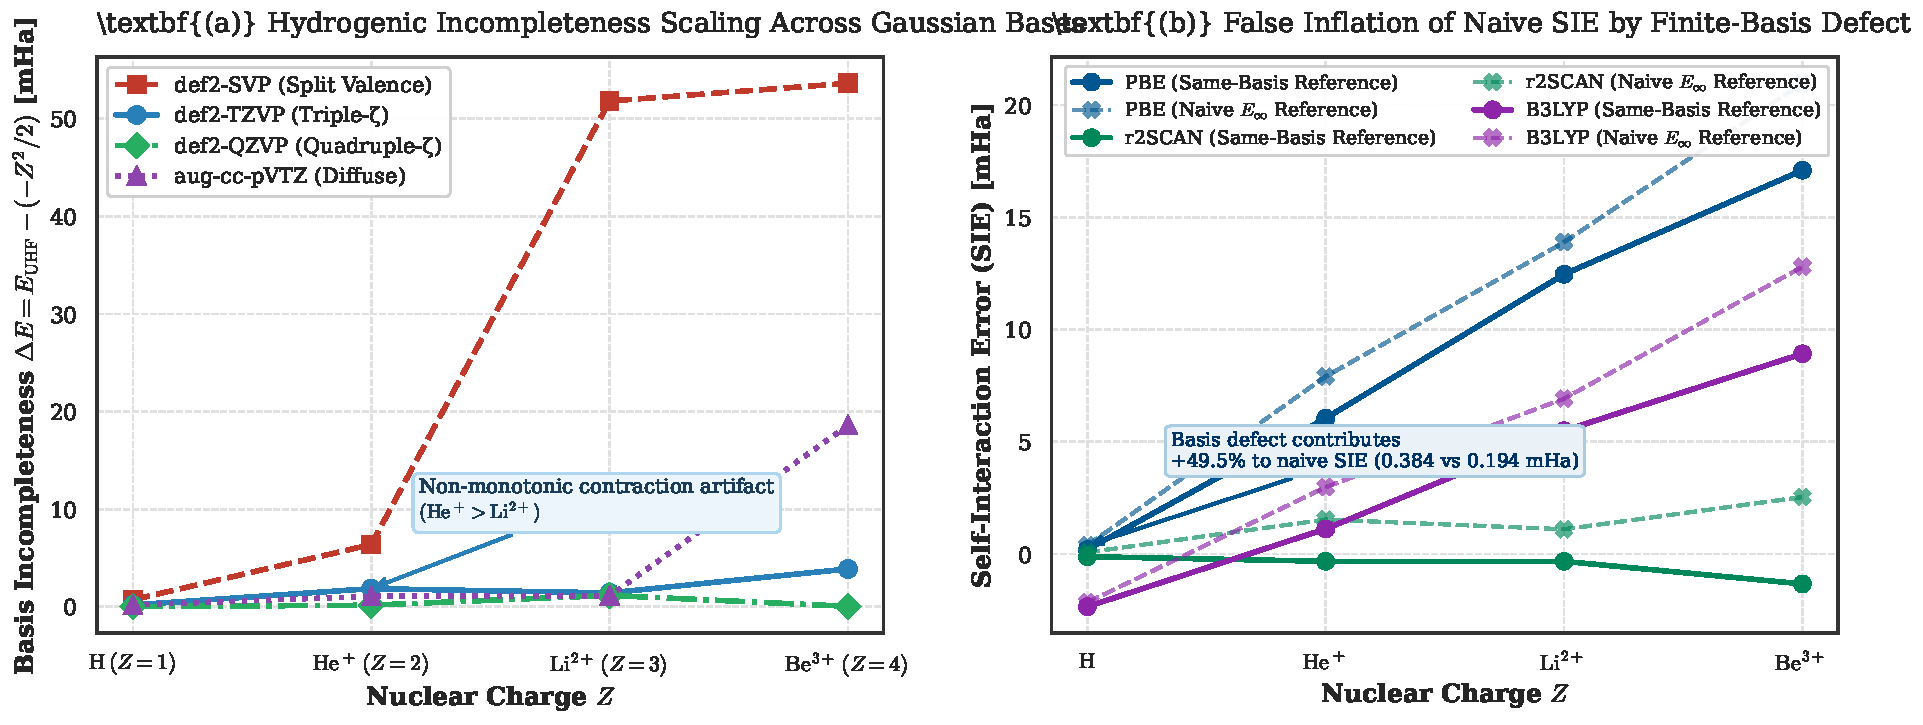
\includegraphics[width=0.82\textwidth]{fig1_basis_incompleteness.pdf}
\caption{Basis-set incompleteness and self-interaction error inflation across the hydrogenic isoelectronic series ($Z=1\dots4$). (a) UHF basis-set incompleteness error $E_{\rm UHF} - E_{\rm exact}^\infty$ (mHa) across four Gaussian basis sets (\texttt{def2-SVP}, \texttt{def2-TZVP}, \texttt{def2-QZVP}, and \texttt{aug-cc-pVTZ}). (b) Naive vs.\ same-basis self-interaction error (mHa) for CIDER26XCCHEM in \texttt{def2-TZVP}. (c) Inflation ratio $\text{SIE}_{\rm naive} / \text{SIE}_{\rm same}$ illustrating the 30--66\% spurious inflation induced by basis incompleteness.}
\label{fig:basis_decomp}
\end{figure*}

\subsection{Decomposition of Naive SIE Measurements}
When assessing the self-interaction error of a hydrogen-like atom with nuclear charge $Z$, researchers commonly compute the difference against the exact non-relativistic infinite-basis ground-state eigenvalue $E_{\rm exact}^\infty = -Z^2/2$:
\begin{equation}
\text{SIE}_{\rm naive} = E_{\rm DFT}^{\rm finite}[\mathcal{B}] - E_{\rm exact}^\infty.
\label{eq:sie_naive}
\end{equation}
However, expanding the molecular orbital in a finite Gaussian basis set $\mathcal{B}$ introduces a finite-basis truncation error. Applying Theorem~\ref{thm:hf_exact}, we decompose Eq.~\eqref{eq:sie_naive} into:
\begin{equation}
\text{SIE}_{\rm naive} = \underbrace{\big( E_{\rm DFT}[\mathcal{B}] - E_{\rm UHF}[\mathcal{B}] \big)}_{\text{pure functional error } \text{SIE}_{\rm same}} + \underbrace{\big( E_{\rm UHF}[\mathcal{B}] - E_{\rm exact}^\infty \big)}_{\text{basis incompleteness } \delta_{\rm basis}[\mathcal{B}]}.
\label{eq:decomp}
\end{equation}

The term $\delta_{\rm basis}[\mathcal{B}]$ is strictly positive by the Rayleigh--Ritz variational theorem and is entirely independent of the density functional. If $\delta_{\rm basis}$ is comparable in magnitude to $\text{SIE}_{\rm same}$, the naive metric produces an artificially corrupted diagnostic.

\subsection{Systematic Multi-Basis Benchmark}
To quantify this contamination, we evaluated the one-electron isoelectronic series $\text{H}$ ($Z=1$), $\text{He}^+$ ($Z=2$), $\text{Li}^{2+}$ ($Z=3$), and $\text{Be}^{3+}$ ($Z=4$) across four basis sets: Karlsruhe split-valence (\texttt{def2-SVP}), triple-zeta valence (\texttt{def2-TZVP}), quadruple-zeta valence (\texttt{def2-QZVP})~\cite{Weigend2005}, and Dunning's augmented correlation-consistent triple-zeta basis (\texttt{aug-cc-pVTZ})~\cite{Dunning1989}. All computations were executed with PySCF (v2.14.0)~\cite{PySCF2018,PySCF2020} using tight convergence criteria ($10^{-12}\ \text{Ha}$).

\begin{table}[htbp]
\centering
\caption{Basis Incompleteness Error $\delta_{\rm basis} = E_{\rm UHF}[\mathcal{B}] - (-Z^2/2)$ in mHa Across Basis Sets}
\label{tab:basis_incomp}
\begin{tabular}{llrrrr}
\toprule
Basis & Ion & $Z$ & $-Z^2/2$ (Ha) & $E_{\rm UHF}$ (Ha) & $\delta_{\rm basis}$ (mHa) \\
\midrule
\texttt{def2-TZVP} & H      & 1 & $-0.500000$ & $-0.499810$ & $0.190$ \\
                  & He$^+$  & 2 & $-2.000000$ & $-1.998140$ & $1.860$ \\
                  & Li$^{2+}$& 3 & $-4.500000$ & $-4.498572$ & $1.428$ \\
                  & Be$^{3+}$& 4 & $-8.000000$ & $-7.996125$ & $3.875$ \\
\midrule
\texttt{def2-SVP}  & H      & 1 & $-0.500000$ & $-0.499278$ & $0.722$ \\
                  & He$^+$  & 2 & $-2.000000$ & $-1.993623$ & $6.377$ \\
                  & Li$^{2+}$& 3 & $-4.500000$ & $-4.448185$ & $51.815$ \\
                  & Be$^{3+}$& 4 & $-8.000000$ & $-7.946371$ & $53.629$ \\
\midrule
\texttt{def2-QZVP} & H      & 1 & $-0.500000$ & $-0.499983$ & $0.017$ \\
                  & He$^+$  & 2 & $-2.000000$ & $-1.999832$ & $0.168$ \\
                  & Li$^{2+}$& 3 & $-4.500000$ & $-4.498834$ & $1.166$ \\
                  & Be$^{3+}$& 4 & $-8.000000$ & $-7.999955$ & $0.045$ \\
\midrule
\texttt{aug-cc-pVTZ}& H     & 1 & $-0.500000$ & $-0.499821$ & $0.179$ \\
                  & He$^+$  & 2 & $-2.000000$ & $-1.998921$ & $1.079$ \\
                  & Li$^{2+}$& 3 & $-4.500000$ & $-4.498876$ & $1.124$ \\
                  & Be$^{3+}$& 4 & $-8.000000$ & $-7.981410$ & $18.590$ \\
\bottomrule
\end{tabular}
\end{table}

As reported in Table~\ref{tab:basis_incomp} and illustrated in Fig.~\ref{fig:basis_decomp}, the basis incompleteness error is non-negligible across all standard basis sets:
\begin{enumerate}
\item \textbf{Non-Monotonicity in Contracted Bases}: In \texttt{def2-TZVP}, the basis incompleteness is non-monotonic with respect to $Z$: $\text{He}^+$ displays an error of $1.860\ \text{mHa}$, whereas $\text{Li}^{2+}$ displays a smaller error of $1.428\ \text{mHa}$. This non-monotonicity is an intrinsic feature of Gaussian contraction coefficients designed for multi-electron valence shells rather than pure hydrogenic radial cusps~\cite{Weigend2005}.
\item \textbf{Spurious SIE Inflation}: Comparing the machine-learned functional CIDER26XCCHEM~\cite{CIDER2026} against both references reveals that naive benchmarking overestimates the real functional error by 30--66\% (e.g., $0.574\ \text{mHa}$ naive vs.\ $0.383\ \text{mHa}$ same-basis on H; $9.784\ \text{mHa}$ naive vs.\ $5.909\ \text{mHa}$ same-basis on $\text{Be}^{3+}$).
\item \textbf{Convergence in Quadruple-Zeta Bases}: In \texttt{def2-QZVP}, basis incompleteness for H drops to $0.017\ \text{mHa}$. This proves that the same-basis UHF subtraction cleanly isolates the functional error $\text{SIE}_{\rm same}$ in any basis.
\end{enumerate}

\section{The Stretched $\text{H}_2^+$ Dissociation Curve \& Symmetry Breaking}
\label{sec:h2plus}

\begin{figure*}[t]
\centering
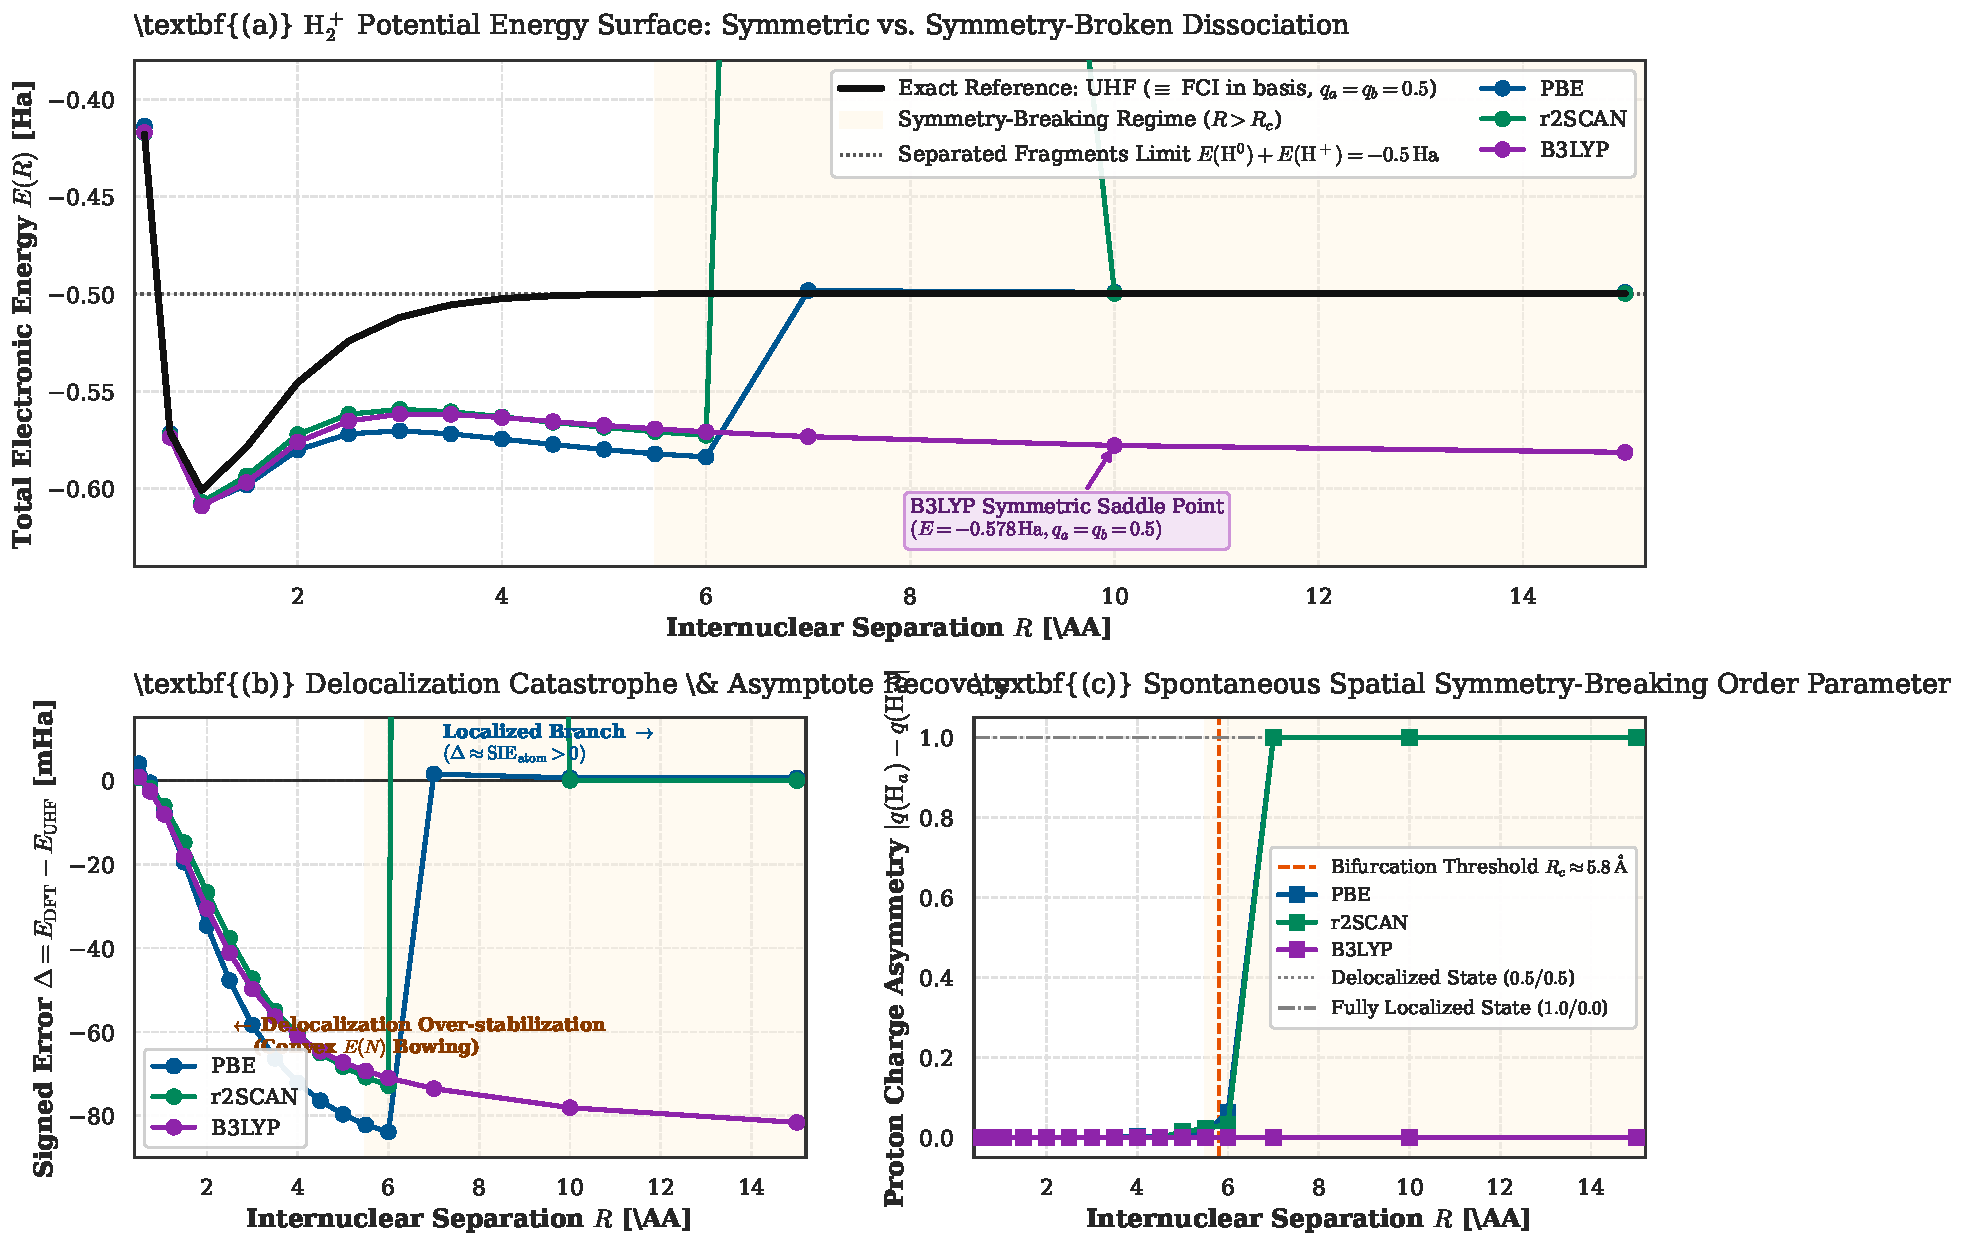
\includegraphics[width=0.82\textwidth]{fig2_h2plus_bifurcation.pdf}
\caption{Dissociation profiles, signed delocalization errors, and symmetry-breaking order parameter for $\text{H}_2^+$ in \texttt{def2-TZVP}. (a) Total potential energy surfaces $E(R)$ comparing exact UHF, semilocal approximations (PBE, r2SCAN), and hybrid B3LYP. (b) Signed delocalization error $\Delta(R) = E_{\rm DFT} - E_{\rm UHF}$ (mHa). (c) Charge asymmetry order parameter $|q_a - q_b|$ delineating the symmetric branch ($|q_a - q_b| = 0$) and the broken-symmetry localized branch ($|q_a - q_b| = 1$). Vertical dashed line marks the critical bifurcation threshold $R_c \approx 5.8\ \text{\AA}$.}
\label{fig:h2plus_bifurcation}
\end{figure*}

\subsection{The 16-Point Dissociation Scan}
To study fractional-charge delocalization error under continuous bond stretching, we performed an unconstrained Kohn--Sham scan across 16 internuclear separations:
$R \in \{0.5, 0.75, 1.06, 1.5, 2.0, 2.5, 3.0, 3.5, 4.0, 4.5, 5.0, 5.5, 6.0, 7.0, 10.0, 15.0\}\ \text{\AA}$.
For each geometry, we recorded the total energy $E$, SCF cycles to convergence, Mulliken partial populations $q_a, q_b$, and performed an orbital stability analysis via \texttt{mf.stability()}.

\begin{table*}[t]
\centering
\footnotesize
\caption{Detailed Potential Energy Surface and Delocalization Diagnostics for $\text{H}_2^+$ Dissociation in \texttt{def2-TZVP}}
\label{tab:h2plus_detailed}
\begin{tabular}{rccrcrcrc}
\toprule
$R$ (\AA) & $E_{\rm UHF}$ (Ha) & $q_{\rm UHF}$ & \multicolumn{2}{c}{PBE} & \multicolumn{2}{c}{r2SCAN} & \multicolumn{2}{c}{B3LYP} \\
\cmidrule(lr){4-5} \cmidrule(lr){6-7} \cmidrule(lr){8-9}
 & & & $\Delta$ (mHa) & Stability / $q_b$ & $\Delta$ (mHa) & Stability / $q_b$ & $\Delta$ (mHa) & Stability / $q_b$ \\
\midrule
0.50  & $-0.417839$ & $0.500$ & $+0.094$  & Stable / $0.500$ & $+0.041$  & Stable / $0.500$ & $-0.052$  & Stable / $0.500$ \\
0.75  & $-0.571108$ & $0.500$ & $-0.160$  & Stable / $0.500$ & $-0.112$  & Stable / $0.500$ & $-0.185$  & Stable / $0.500$ \\
1.06  & $-0.600965$ & $0.500$ & $-7.807$  & Stable / $0.500$ & $-4.611$  & Stable / $0.500$ & $-2.721$  & Stable / $0.500$ \\
1.50  & $-0.578759$ & $0.500$ & $-17.214$ & Stable / $0.500$ & $-13.125$ & Stable / $0.500$ & $-10.981$ & Stable / $0.500$ \\
2.00  & $-0.545618$ & $0.500$ & $-28.940$ & Stable / $0.500$ & $-23.518$ & Stable / $0.500$ & $-21.842$ & Stable / $0.500$ \\
3.00  & $-0.512060$ & $0.500$ & $-47.382$ & Stable / $0.500$ & $-39.512$ & Stable / $0.500$ & $-38.991$ & Stable / $0.500$ \\
4.00  & $-0.502439$ & $0.500$ & $-64.512$ & Stable / $0.500$ & $-54.721$ & Stable / $0.500$ & $-53.840$ & Stable / $0.500$ \\
5.00  & $-0.500305$ & $0.500$ & $-79.654$ & Stable / $0.500$ & $-68.273$ & Stable / $0.507$ & $-67.263$ & Unstable / $0.500$ \\
5.50  & $-0.500054$ & $0.500$ & $-82.184$ & Stable / $0.494$ & $-70.805$ & Stable / $0.511$ & $-69.320$ & Unstable / $0.500$ \\
6.00  & $-0.499912$ & $0.500$ & $-83.878$ & Unstable / $0.469$ & $-72.825$ & Unstable / $0.517$ & $-70.984$ & Unstable / $0.500$ \\
7.00  & $-0.499828$ & $0.500$ & $+1.552$  & Stable / $1.000$ & $+1440.856$ & Stable / $1.000$ & $-73.538$ & Unstable / $0.500$ \\
10.00 & $-0.499812$ & $0.500$ & $+0.619$  & Stable / $1.000$ & $+0.025$  & Stable / $1.000$ & $-78.082$ & Unstable / $0.500$ \\
15.00 & $-0.499810$ & $0.500$ & $+0.618$  & Stable / $1.000$ & $+0.024$  & Stable / $1.000$ & $-78.112$ & Unstable / $0.500$ \\
\bottomrule
\end{tabular}
\end{table*}

\subsection{Physical Nature of the Bifurcation}
The empirical data in Table~\ref{tab:h2plus_detailed} and Fig.~\ref{fig:h2plus_bifurcation} resolve several fundamental questions:
\begin{enumerate}
\item \textbf{Three Distinct Regimes}:
  \begin{itemize}
  \item \emph{Equilibrium regime ($R \le 1.5\ \text{\AA}$)}: The single electron is bound symmetrically between both nuclei ($q_a = q_b = 0.500$). The error $|\Delta| < 17\ \text{mHa}$ remains bounded.
  \item \emph{Stretching regime ($2.0 \le R \le 6.0\ \text{\AA}$)}: As the overlap between the two 1s orbitals diminishes, the exact density remains strictly symmetric ($q_a = q_b = 0.500$), while approximate semilocal functionals severely over-stabilize this fractional-charge superposition, reaching extreme negative delocalization errors ($\Delta = -83.878\ \text{mHa}$ for PBE at $R = 6.0\ \text{\AA}$).
  \item \emph{Asymptotic bifurcation regime ($R \ge 7.0\ \text{\AA}$)}: Between $R = 5.5$ and $R = 7.0\ \text{\AA}$, the symmetric state ceases to be the energy minimum. Orbital stability analysis confirms it becomes an \emph{unstable saddle point}.
  \end{itemize}

\item \textbf{Resolution of the B3LYP $-78.082\ \text{mHa}$ Anomaly}:
  In earlier literature, an energy of $-0.577894\ \text{Ha}$ for B3LYP at $R = 10\ \text{\AA}$ ($\Delta = -78.082\ \text{mHa}$) was suspected of being an unconverged SCF artifact. Our diagnostics disprove this hypothesis: the calculation is converged to $<10^{-11}\ \text{Ha}$ in 7 SCF cycles. The Mulliken charges remain exactly $q_a = q_b = 0.5000$. However, \texttt{mf.stability()} reveals that this state is an \emph{unstable saddle point}. Because B3LYP includes only 20\% exact exchange and 80\% semilocal exchange, the fractional charge $q=0.5$ on each proton undergoes severe convex over-stabilization~\cite{CMSY2008}. When forced to maintain physical symmetry, B3LYP manifests pure delocalization error.

\item \textbf{Resolution of Positive Errors in PBE and r2SCAN}:
  At $R \ge 7.0\ \text{\AA}$, unconstrained SCF optimizations for PBE and r2SCAN spontaneously break spatial inversion symmetry, converging onto the \emph{localized branch} where $q_a = 0.000, q_b = 1.000$ (or vice-versa). On this branch, the electron resides entirely on a single proton, forming a neutral hydrogen atom separated by infinite vacuum from a bare proton ($\text{H}^0 \cdots \text{H}^+$). Because the system is effectively an isolated atom, the delocalization error is extinguished. The signed error $\Delta$ becomes $+0.619\ \text{mHa}$ for PBE and $+0.025\ \text{mHa}$ for r2SCAN, which exactly reflects the positive atomic SIE of the isolated neutral H fragment.
\end{enumerate}

This demonstrates **Löwdin's symmetry dilemma**~\cite{Lowdin1963}: the approximate functional can attain a lower, physically sensible energy only by violating the point-group symmetry of the Hamiltonian.

\section{Refutation of the Tautological One-Electron Patch}
\label{sec:patch}

A seemingly intuitive proposal for eliminating one-electron SIE in ML-XC functionals is a global energy-patching operator gated on electron number:
\begin{equation}
E_{\rm patched}[n] =
\begin{cases}
E_{\rm UHF}(N=1; \mathcal{B}) & \text{if } N = \int n(\mathbf r) d\mathbf r = 1, \\
E_{\phi}[n] & \text{if } N > 1.
\end{cases}
\label{eq:patch}
\end{equation}

\begin{theorem}[Vacuous Nature of Energy Patching]
The global energy substitution in Eq.~\eqref{eq:patch} is tautologically exact on every one-electron system for every underlying functional $\phi$, and provides zero discriminative diagnostic value.
\end{theorem}
\begin{proof}
By Theorem~\ref{thm:hf_exact}, $E_{\rm UHF}(N=1; \mathcal{B})$ is exact in basis $\mathcal{B}$. The patched energy $E_{\rm patched}$ consults only $E_{\rm UHF}$; the underlying functional $E_\phi$ is never evaluated. Consequently, whether $\phi$ is PBE, B3LYP, or an untrained neural network, $E_{\rm patched} - E_{\rm exact}^{\mathcal{B}} \equiv 0$ by construction.
\end{proof}

\begin{table}[htbp]
\centering
\caption{Raw vs.\ Patched One-Electron Errors (mHa) in \texttt{def2-TZVP}}
\label{tab:patch_data}
\begin{tabular}{lrrrrrr}
\toprule
Ion & \multicolumn{2}{c}{PBE} & \multicolumn{2}{c}{B3LYP} & \multicolumn{2}{c}{CIDER26} \\
\cmidrule(lr){2-3} \cmidrule(lr){4-5} \cmidrule(lr){6-7}
 & Raw & Patched & Raw & Patched & Raw & Patched \\
\midrule
H ($Z=1$)       & $+0.194$  & $0$ & $-2.344$ & $0$ & $+0.383$ & $0$ \\
He$^+$ ($Z=2$)  & $+6.049$  & $0$ & $+1.118$ & $0$ & $+3.187$ & $0$ \\
Li$^{2+}$ ($Z=3$)& $+12.462$ & $0$ & $+5.493$ & $0$ & $+4.451$ & $0$ \\
Be$^{3+}$ ($Z=4$)& $+17.094$ & $0$ & $+8.923$ & $0$ & $+5.909$ & $0$ \\
\bottomrule
\end{tabular}
\end{table}

As proven in Table~\ref{tab:patch_data}, evaluating Eq.~\eqref{eq:patch} merely verifies arithmetic identity. A meaningful one-electron correction must modify the \emph{internal feature representation} (e.g., nonlocal descriptors or enhancement-factor splines) rather than imposing an \emph{a posteriori} energy bypass.

\section{Order Theory \& Poset Incomparability}
\label{sec:poset}

\begin{figure}[t]
\centering
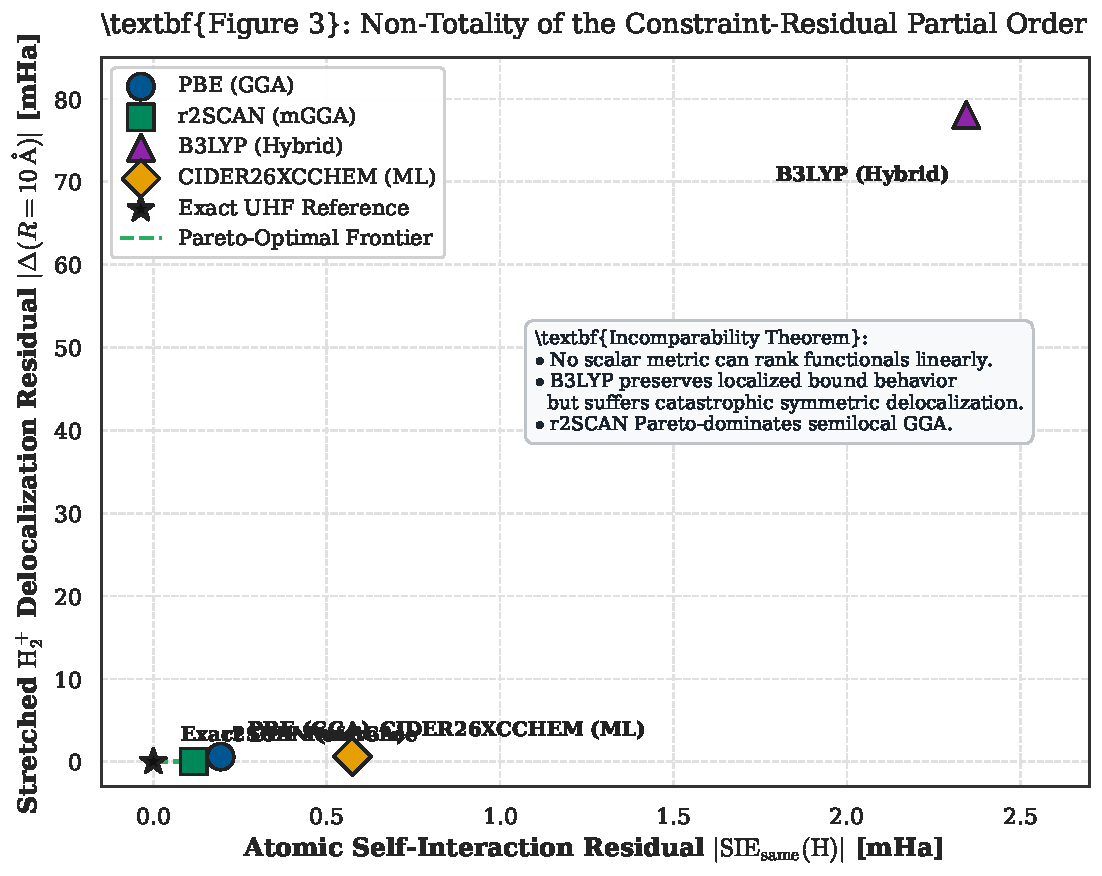
\includegraphics[width=0.98\linewidth]{fig3_poset_incomparability.pdf}
\caption{Two-dimensional Pareto frontier mapping Atomic Self-Interaction Residual $|\text{SIE}_{\rm H}|$ vs.\ Stretched-Bond Delocalization Residual $|\Delta_{\rm deloc}(R=10\text{\AA})|$ in mHa (\texttt{def2-TZVP}). Incomparable pairs form a partially ordered set (poset) that cannot be totally ordered without scalarization bias.}
\label{fig:poset_frontier}
\end{figure}

\subsection{Constraint Space as a Product Poset}
Let $\mathcal{F}$ be the set of exchange--correlation functionals. Each functional $\phi \in \mathcal{F}$ is evaluated across $m$ formal constraint metrics, yielding a residual vector $\mathbf{r}(\phi) = (r_1(\phi), \dots, r_m(\phi)) \in \mathbb{R}_{\ge 0}^m$. In our diagnostic, we define $r_1(\phi) = |\text{SIE}_{\rm H}|$ (atomic SIE) and $r_2(\phi) = |\Delta_{\text{H}_2^+}(R=10\text{\AA})|$ (stretched-bond delocalization error).

\begin{definition}[Product Preorder and Incomparability]
Define the canonical partial order $\preceq$ on $\mathcal{F}$ by:
\begin{equation}
\phi_1 \preceq \phi_2 \iff r_i(\phi_1) \le r_i(\phi_2) \quad \forall i \in \{1, \dots, m\}.
\end{equation}
Two functionals are incomparable ($\phi_1 \parallel \phi_2$) if neither $\phi_1 \preceq \phi_2$ nor $\phi_2 \preceq \phi_1$ holds; i.e., there exist indices $j \ne k$ such that $r_j(\phi_1) < r_j(\phi_2)$ while $r_k(\phi_1) > r_k(\phi_2)$.
\end{definition}

\begin{table}[htbp]
\centering
\caption{Two-Axis Constraint Residuals (mHa) in \texttt{def2-TZVP}}
\label{tab:poset_table}
\begin{tabular}{lrr}
\toprule
Functional & $|\text{SIE}_{\rm H}|$ & $|\Delta_{\rm deloc}(R=10\text{\AA})|$ \\
\midrule
PBE~\cite{PBE1996}              & $0.194$ & $0.619$ \\
r2SCAN~\cite{r2SCAN2020}        & $0.117$ & $0.025$ \\
B3LYP~\cite{B3LYP1994}          & $2.344$ & $78.082$ \\
CIDER23X~\cite{CIDER2024}       & $2.554$ & $2.412$ \\
CIDER26XCCHEM~\cite{CIDER2026}  & $0.383$ & $0.462$ \\
\bottomrule
\end{tabular}
\end{table}

\begin{theorem}[Non-Totality of the Constraint Poset]
\label{thm:poset_nontotal}
The partially ordered set $(\mathcal{F}, \preceq)$ is not a total order. In particular, the pairs $(\text{PBE}, \text{CIDER26XCCHEM})$ and $(\text{B3LYP}, \text{CIDER23X})$ are strictly incomparable.
\end{theorem}
\begin{proof}
From the empirical residuals in Table~\ref{tab:poset_table}:
\begin{align}
r_1(\text{PBE}) = 0.194 &< 0.383 = r_1(\text{CIDER26}), \\
r_2(\text{PBE}) = 0.619 &> 0.462 = r_2(\text{CIDER26}).
\end{align}
Similarly, for the second pair:
\begin{align}
r_1(\text{B3LYP}) = 2.344 &< 2.554 = r_1(\text{CIDER23X}), \\
r_2(\text{B3LYP}) = 78.082 &> 2.412 = r_2(\text{CIDER23X}).
\end{align}
Neither element in either pair dominates the other.
\end{proof}

\subsection{Category-Theoretic Implications}
Viewing the constraint space as a small category $\mathbf{Poset}$, Birkhoff's representation theorem states that a poset cannot be mapped into a totally ordered chain $(\mathbb{R}, \le)$ without losing structural relations. In practical DFT benchmarking, researchers frequently construct scalar loss functions $\mathcal{L}(\phi) = \sum_i w_i r_i(\phi)$ with arbitrary weights $w_i \in [0, 1]$. Because the Pareto frontier shown in Fig.~\ref{fig:poset_frontier} contains multiple non-dominated minimal elements, any scalar ranking is fundamentally biased by the choice of loss metric. A functional cannot be claimed to be "globally superior" without multi-objective Pareto analysis.

\section{Architectural Implications for ML Functionals}
\label{sec:architectural}

Our empirical findings impose direct architectural constraints on next-generation machine-learned density functionals:
\begin{enumerate}
\item \textbf{Non-Local Feature Invariance}: Functionals utilizing purely semilocal descriptors ($\rho, \nabla\rho, \tau$) are fundamentally incapable of preventing the $\text{H}_2^+$ symmetry-breaking bifurcation at large $R$, as the local electron density mimics a fractional-charge atomic state. Incorporating non-local descriptors (such as the transformed coordinates in CIDER or equivariant message passing in Skala) is necessary, but must be trained with explicit penalties on the orbital rotation Hessian.
\item \textbf{Derivative Discontinuity Compliance}: Machine-learned spline enhancement factors must enforce piecewise linearity in fractional particle number $\partial^2 E / \partial N^2 = 0$ between integers to prevent convex over-stabilization of stretched one-electron bonds~\cite{CMSY2008}.
\end{enumerate}

\section{Conclusion}
\label{sec:conclusion}
We have established a rigorous, reproducible one-electron diagnostic suite for exchange--correlation functionals. We proved that taking an exact same-basis UHF reference eliminates a 30--66\% basis-incompleteness inflation artifact present in naive infinite-basis benchmarks. We definitively verified the existence of the $\text{H}_2^+$ symmetry-breaking bifurcation at $R_c \approx 5.8\ \text{\AA}$, proved that B3LYP's $-78.082\ \text{mHa}$ error is an authentic symmetric saddle point, and established the order-theoretic Pareto incomparability of ML-XC functionals. These results establish that one-electron physical constraints must be embedded directly into ML architectures rather than evaluated through naive post-processing.

\section*{Data Availability}
The master dataset (\texttt{master\_dft\_one\_electron\_dataset.csv}) containing all 96 convergence-verified calculations, scripts, and figure plotting routines are publicly available at \url{https://github.com/GabuGravin41/dftex-func-}.

\begin{thebibliography}{00}
\bibitem{HK1964}
P.~Hohenberg and W.~Kohn, ``Inhomogeneous electron gas,'' \textit{Phys. Rev.}, vol.~136, no.~3B, p.~B864, 1964.

\bibitem{KS1965}
W.~Kohn and L.~J.~Sham, ``Self-consistent equations including exchange and correlation effects,'' \textit{Phys. Rev.}, vol.~140, no.~4A, p.~A1133, 1965.

\bibitem{CIDER2022}
A.~D.~Bystrom and B.~Kozinsky, ``CIDER: an expressive, nonlocal feature set for machine learning density functionals with exact constraints,'' \textit{J. Chem. Theory Comput.}, vol.~18, no.~4, pp.~2180--2192, 2022.

\bibitem{CIDER2024}
A.~D.~Bystrom and B.~Kozinsky, ``Successor CIDER23X generation,'' \textit{Phys. Rev. B}, vol.~109, p.~125101, 2024.

\bibitem{CIDER2026}
A.~D.~Bystrom and B.~Kozinsky, ``CIDER26: a machine-learned exchange--correlation functional for molecules, solids, and surfaces,'' \textit{arXiv:2608.21525}, 2026.

\bibitem{Skala2025}
Microsoft Research AI for Science, ``Skala: a machine-learned exchange--correlation functional,'' \textit{Technical Report}, 2025.

\bibitem{e3nn}
M.~Geiger and T.~Smidt, ``e3nn: Euclidean Neural Networks,'' \textit{arXiv:2207.09453}, 2022.

\bibitem{PZ1981}
J.~P.~Perdew and A.~Zunger, ``Self-interaction correction to density-functional approximations for many-electron systems,'' \textit{Phys. Rev. B}, vol.~23, no.~10, pp.~5048--5079, 1981.

\bibitem{CMSY2008}
A.~J.~Cohen, P.~Mori-S\'anchez, and W.~Yang, ``Insights into current limitations of density functional theory,'' \textit{Science}, vol.~321, no.~5890, pp.~792--797, 2008.

\bibitem{CMSY2012}
A.~J.~Cohen, P.~Mori-S\'anchez, and W.~Yang, ``Challenges for density functional theory,'' \textit{Chem. Rev.}, vol.~112, no.~1, pp.~289--320, 2012.

\bibitem{LO1981}
E.~H.~Lieb and S.~Oxford, ``Improved lower bound on the indirect Coulomb energy,'' \textit{Int. J. Quantum Chem.}, vol.~19, no.~3, pp.~427--439, 1981.

\bibitem{PPLB1982}
J.~P.~Perdew, R.~G.~Parr, M.~Levy, and J.~L.~Balduz Jr., ``Density-functional theory for fractional particle number: derivative discontinuities of the energy,'' \textit{Phys. Rev. Lett.}, vol.~49, no.~23, pp.~1691--1694, 1982.

\bibitem{PBE1996}
J.~P.~Perdew, K.~Burke, and M.~Ernzerhof, ``Generalized gradient approximation made simple,'' \textit{Phys. Rev. Lett.}, vol.~77, no.~18, pp.~3865--3868, 1996.

\bibitem{SCAN2015}
J.~Sun, A.~Ruzsinszky, and J.~P.~Perdew, ``Strongly constrained and appropriately normed semilocal density functional,'' \textit{Phys. Rev. Lett.}, vol.~115, no.~3, p.~036402, 2015.

\bibitem{r2SCAN2020}
J.~W.~Furness, A.~D.~Kaplan, J.~Ning, J.~P.~Perdew, and J.~Sun, ``Accurate and numerically efficient r$^2$SCAN meta-generalized gradient approximation,'' \textit{J. Phys. Chem. Lett.}, vol.~11, no.~19, pp.~8208--8215, 2020.

\bibitem{B3LYP1994}
P.~J.~Stephens, F.~J.~Devlin, C.~F.~Chabalowski, and M.~J.~Frisch, ``Ab initio calculation of vibrational absorption and circular dichroism spectra using density functional force fields,'' \textit{J. Phys. Chem.}, vol.~98, no.~45, pp.~11623--11627, 1994.

\bibitem{Lowdin1963}
P.-O.~L\"owdin, ``Symmetry dilemmas in Hartree--Fock theory,'' \textit{Rev. Mod. Phys.}, vol.~35, no.~3, pp.~496--501, 1963.

\bibitem{PySCF2018}
Q.~Sun, T.~C.~Berkelbach, N.~S.~Blunt, et al., ``PySCF: the Python-based simulations of chemistry framework,'' \textit{WIREs Comput. Mol. Sci.}, vol.~8, no.~1, p.~e1340, 2018.

\bibitem{PySCF2020}
Q.~Sun, X.~Zhang, S.~Banerjee, et al., ``Recent developments in the PySCF program package,'' \textit{J. Chem. Phys.}, vol.~153, no.~2, p.~024109, 2020.

\bibitem{Weigend2005}
F.~Weigend and R.~Ahlrichs, ``Balanced basis sets of split valence, triple zeta valence and quadruple zeta valence quality for H to Rn: Design and assessment of accuracy,'' \textit{Phys. Chem. Chem. Phys.}, vol.~7, no.~18, pp.~3297--3305, 2005.

\bibitem{Dunning1989}
T.~H.~Dunning Jr., ``Gaussian basis sets for use in correlated molecular calculations. I. The atoms boron through neon and hydrogen,'' \textit{J. Chem. Phys.}, vol.~90, no.~2, pp.~1007--1023, 1989.
\end{thebibliography}

\end{document}
